\documentclass{article}
\usepackage{bigstrut}
\usepackage{adjustbox}
\usepackage{graphicx}^^M
\graphicspath{ {images/} }
\usepackage[T1]{fontenc}
\usepackage{float}

\usepackage[english]{babel}
\usepackage[utf8]{inputenc}
\usepackage{indentfirst}

\addtolength{\oddsidemargin}{-.875in}
\addtolength{\evensidemargin}{-.875in}
\addtolength{\textwidth}{1.75in}
\addtolength{\textheight}{1in}

\begin{document}
\title{Design V: Lab 5}
\begin{titlepage}
    \centering
	{\scshape\LARGE Lab 5: Heat Treatment\par}
	\vspace{1cm}
	{\scshape Alex Smith: Recorder \hfill ID\#:10416940 \par}
	{\scshape Marcin Wisniowski: Manager \hfill ID\#:10417225\par}
	{\scshape Naomi Henderson: Technician \hfill ID\#:10406469\par}
    \vfill
	{\scshape Design V, Week 8\par}
	\vspace{.5cm}
	{\scshape Laboratory Performed: March 20th, 2018\\Stevens Institute of Technology\\E-231 Section I Group 1\par}
	\vspace{.5cm}
	{\scshape supervised by\\Mr. Di Wu, Mr. Kai Zong \par}
    \vfill
% Bottom of the page
	{\scshape“I pledge my honor that I have abided by the Stevens Honor System.”\par}
	\vspace{.5cm}
	{\scshape Alex Smith \hfill Date: 03/27/18\\Marcin Wisniowski \hfill Date: 03/27/18\\ Naomi Henderson \hfill Date: 03/27/18\\}
	\vspace{3cm}
\end{titlepage}

\section{Introduction}
In this lab, the group was tasked to compare different cooling treatments of steel and understand how the micro structures changed through each process. Steels are among the most important engineering materials. Perhaps the most important property of steel is the ability to alter its hardness by simple heat treatments and annealment. Following suitable heat treatments hardened steel is highly wear and abrasions resistant and capable of cutting and shaping other softer materials. Steel has multiple different stable phases that it can take the properties of. For different combinations of temperature and pressure, different types of phases can appear in the steel worked on. 


\subsection{Objectives}
\begin{enumerate}
\item Relate thermal processing history to changes in steel microstructure and properties
\item Use photomicroscopy to identify and quantify the percentage of phases in a multiphase microstructure.
\item Use a TTT diagram to design cooling treatments to achieve particular steel microstructures and properties
\end{enumerate}

\subsection{Hypothesis}
The group believes that similar to the effects of annealing in aluminum, the hardness of the steel will decrease when annealed for both samples. The group believes that the sample annealed at a higher temperature will have a lower hardness, as the molecules will arrange differently. The group also believes that a pearlitic steel will have a lower hardness than a martensitic steel because martensite is far less structured.



\section{Procedure}
\subsection{Quenching Hot Steel to Form Martensite}
The group is provided with two small coupons of fully annealed O1 Tool Steel. Each of them is placed through a Rockwell hardness machine to determine its hardness through an average of five samples across the coupon. Later, the steel is wrapped in aluminum foil along with charcoal. The coupons are then placed into a furnace at 825$^oC$ for 30 minutes. One sample is taken out right after the thirty minutes, while the other is transferred over to another furnace at 550$^oC$ for 10 minutes. The samples are both quenched quickly in water after being taken out. Finally, new measurements of hardness are made through the averaging of five different tests across its surface. 

\subsection{Analysis of Steel Microstructures}
Multiple samples of steel are given to the students that all austenitized with time intervals of being quenched in lead at 677$^oC$. This allows a different type of steel to be made, called pearlite due to the temperature.  Using an optical microscope, the percentage of pearlite is estimated for each of the sets. Likewise, multiple pictures of each of the samples is taken for future analysis. 

\section{Results}
Sample 1: 850o C for 40 minutes -> cold water
Sample 2: 850o C for 40 minutes -> 450o C for 10 minutes ->  cold water

\begin{center}
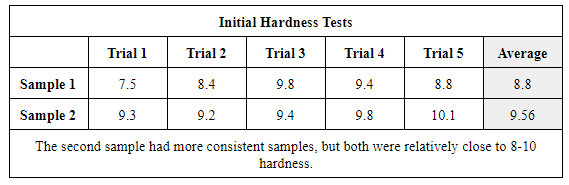
\includegraphics[width=350pt]{1.png}
\end{center}

\begin{center}
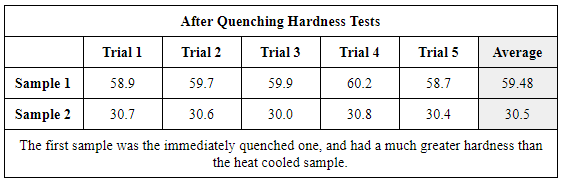
\includegraphics[width=350pt]{2.png}
\end{center}

\begin{center}
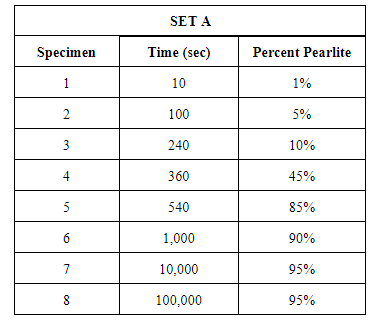
\includegraphics[width=250pt]{3.png}
\end{center}

\begin{center}
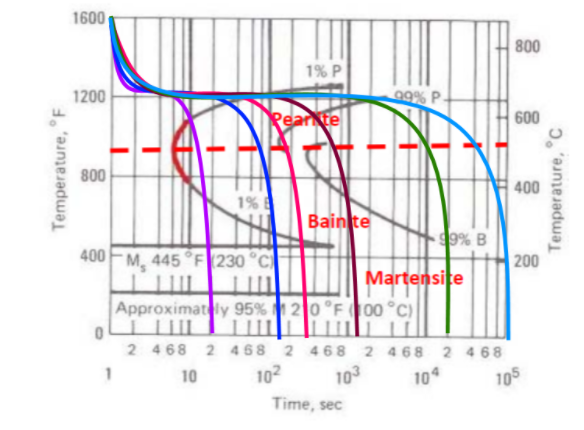
\includegraphics[width=350pt]{4.png}
\end{center}

\newpage 
Set A Images:
\begin{center}
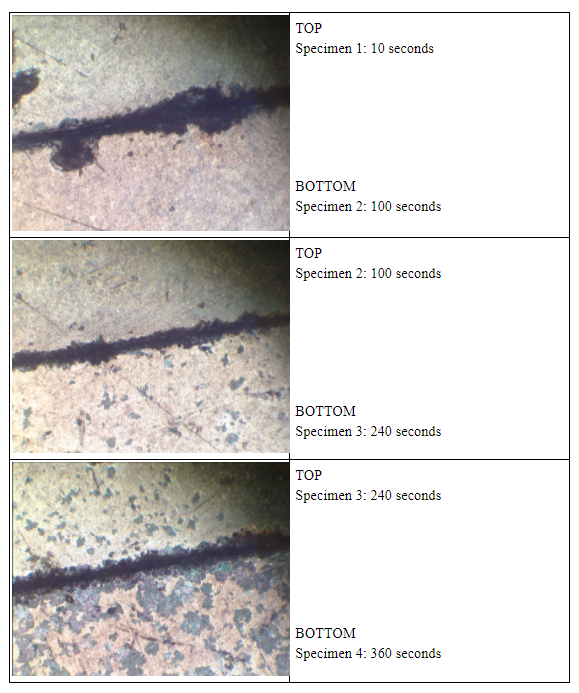
\includegraphics[width=400pt]{5.png}
\end{center}


\begin{center}
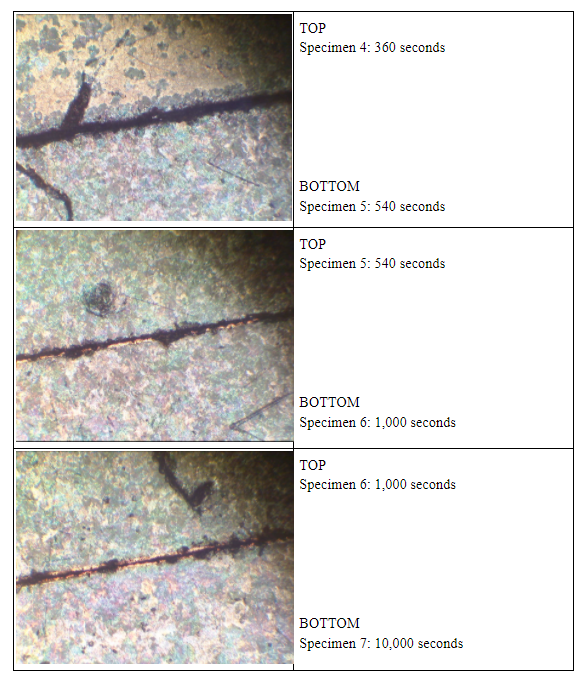
\includegraphics[width=400pt]{6.png}
\end{center}

\begin{center}
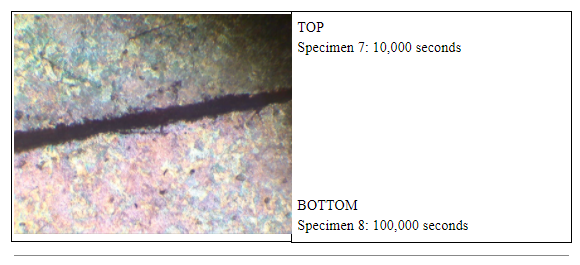
\includegraphics[width=400pt]{7.png}
\end{center}

\begin{center}
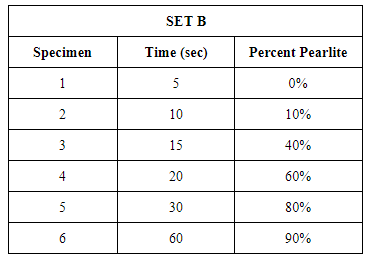
\includegraphics[width=250pt]{9.png}
\end{center}

\newpage 
Set B Images:
\begin{center}
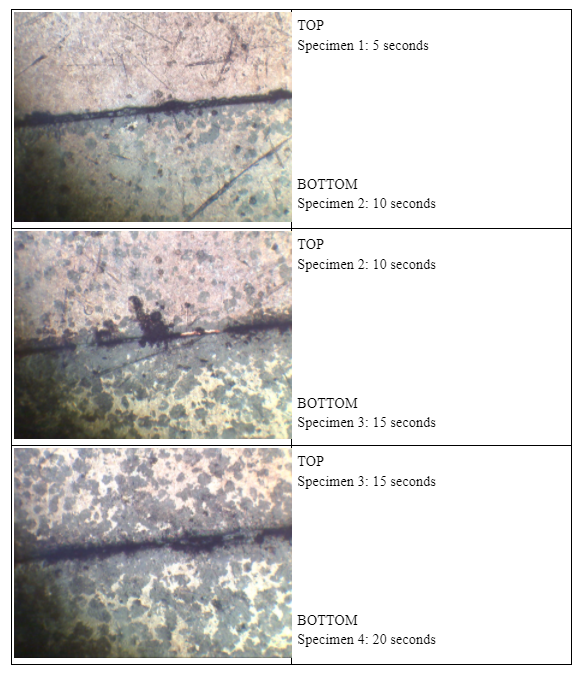
\includegraphics[width=400pt]{10.png}
\end{center}

\begin{center}
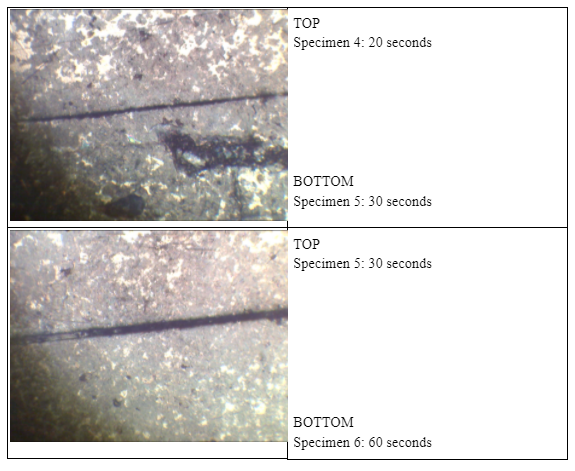
\includegraphics[width=400pt]{11.png}
\end{center}

\begin{center}
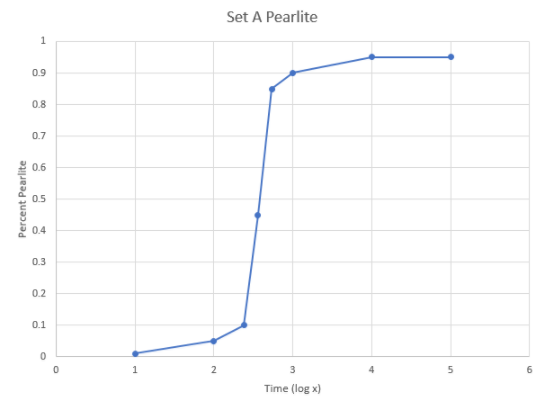
\includegraphics[width=400pt]{12.png}
\end{center}

\begin{center}
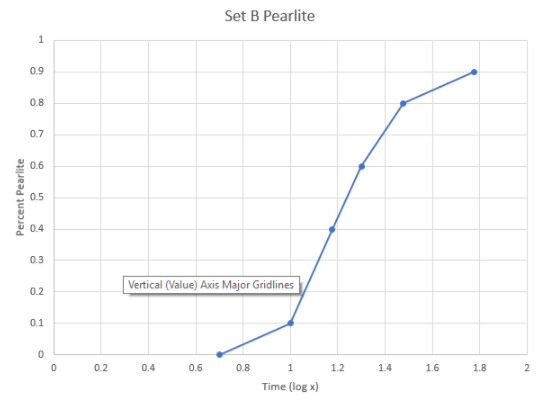
\includegraphics[width=400pt]{14.png}
\end{center}




\section{Discussion}
The group learned throughout this lab that steel, and other materials can be altered in properties by different methods of cooling at different temperatures and time scales. In this lab, the group explored how steel could be changed into a harder or softer material based on how long it sat at a specific temperature before cooling back to room temperature. Not only did this change the final hardness by a large factor, but it even varied in the optical microscope observations through very small or larger time factors. Due to this, metallurgists are able to control the properties of steel in a stable environment as long as they follow precise instructions.
	Still, simply through the process of heat treating an annealed steel coupon, the hardness was convincingly able to rise each time. Based on different amounts of time in different tables, the steel was able to take on many different percentages of pearlite in the optical microscope samples. In Set A, the sample had a very steep curve of increasing pearlite when plotted versus log heat treatment time. Similarly, Set B had a steep curve, but not enough samples to appear as steep in the scale used. By using a TTT diagram for O1 Steel, the estimated observations of pearlite could be plotted onto a graph to see how accurately the observations were made. These steep curves can be seen in the small time difference between \% P and 99\% P as seen on the TTT graph. Even at their maximum, they only vary from 1\% and 99\% by 100 seconds of time. This is apparent in Set B, which austentizes within the bounds relatively quickly.


\section{Broader Impacts}
\begin{enumerate}
\item According to Part A, the fully annealed steel gave a baseline hardness value that only increased with the heat treatment. The pearlitic steel formed by heat cooling provided a modest improvement in hardness. Meanwhile, the martensitic steel formed by water cooling was made of a microstructure of steel that was unable to settle into a softer equilibrium form, and thus was the strongest tested variety. Based on these results, it stands to reason that the samples in Part B will have increasing hardness with increasing pearlitic behavior, as those will exhibit stronger tendencies than the annealed samples.

\item Heat treatment is crucial in the application of steel alloys because it greatly increases the structural stability and durability of the material. Without some form of mechanical processing, the steel samples would not be strong enough to withstand the extreme stresses of commercial applications. Heat treating steel is critical to making those alloys viable in construction and manufacturing processes, as well as relieve structural integrity issues that may make the steel unusable. Martensitic steel is preferred in structural applications when harder materials are needed, and annealed steel is preferred in scenarios when ductility is valued over hardness.
\end{enumerate}

\section{References}
\begin{enumerate}
\item “Metal Hardening / Metal Quenching / Metal Tempering.” Hardening, Quenching, Tempering at 
Metlab of Wyndmoor PA., www.metlabheattreat.com/metal-hardening-metal-quenching-metal-tempering.html.

\item Reshift Media. “Difference Between Annealing and Tempering.” Metal Supermarkets - Steel, 
Aluminum, Stainless, Hot-Rolled, Cold-Rolled, Alloy, Carbon, Galvanized, Brass, Bronze, Copper, 9 May 2016, www.metalsupermarkets.com/difference-annealing-tempering/.

\item “Stainless Steel - Heat Treatment.” AZoM.com, 14 June 2017, 
www.azom.com/article.aspx?ArticleID=1141.

\end{enumerate}

\end{document}